\documentclass[10pt]{article}
\usepackage{pgf,tikz}
\usetikzlibrary{arrows}
\pagestyle{empty}
\begin{document}

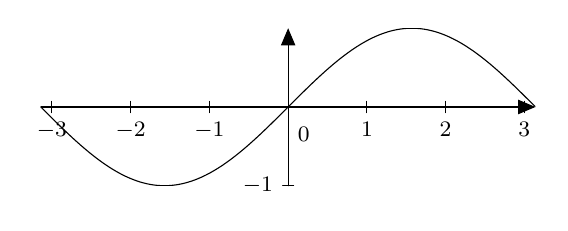
\begin{tikzpicture}[line cap=round,line join=round,>=triangle 45,x=1cm,y=1cm]
	\draw[->,color=black] (-3.14,0) -- (3.14,0);
	\foreach \x in {-3,-2,-1,1,2,3}
	\draw[shift={(\x,0)},color=black] (0pt,2pt) -- (0pt,-2pt) node[below] {\footnotesize $\x$};
	\draw[->,color=black] (0,-1) -- (0,1);
	\foreach \y in {-1}
	\draw[shift={(0,\y)},color=black] (2pt,0pt) -- (-2pt,0pt) node[left] {\footnotesize $\y$};
	\draw[color=black] (0pt,-10pt) node[right] {\footnotesize $0$};
	\clip(-3.14,-1) rectangle (3.14,1);
	\draw[smooth,samples=100,domain=-3.14:3.14] plot(\x,{sin(((\x))*180/pi)});
\end{tikzpicture}

\end{document}
